\chapter{Introduction} \label{introducao}
The research area of autonomous vehicles (AV) is multidisciplinary. With the way the vehicle is built, it is possible to create high impact applications, which establish interrelations and information flows and detect new extended stimuli in scenarios where the infrastructure is physical or mobile \cite{bayat2017environmental}. With this, there is the possibility to apply the concepts of computer vision, which allows the car to see the external environment. Combined with Machine Learning (ML) tools, the vehicle begins to interpret what is around it \cite{rasouli2019autonomous}.

One of the significant challenges of AV detects the position of the car along the road. It is possible to perform this task using the vehicle to infrastructure (V2I) or other techniques such as GPS \cite{hobert2015enhancements}. Therefore, there are some studies to investigate the acceptation of the AV, and a way to prove this new technology can reduce the car accidents, as research guided by Xu et al. where Of the respondents, 42.35\% and 45.28\% expect lower risk and lower insurance premiums for autonomous vehicles, respectively \cite{xu2019autonomous}.

Considering that it is possible to have cameras around the road, in this thesis, we propose an object detection model using multi-cameras. There is a responsible algorithm for detecting and classifying objects, as well as estimating the distance that the position of the object.

\section{Motivation}

The autonomous vehicles are the new reality for the next years with this premise, the new solutions need to grow, and one of these necessities is the vehicle tracking, and should reduce the traffic jams and decrease the number of cars crash \cite{bonnefon2016social}. Given that, there are many levels of self-drive car automation, as shown in Figure \ref{fig:automation}. This work proposes the test scenario of driving automation. To perform tests with drones require much battery during the trial and limit it to 30 to 45 minutes, the proposal is to use the infrastructure along the road as a camera on the pole and send the data to a command center.

\begin{figure}[H]
\centering
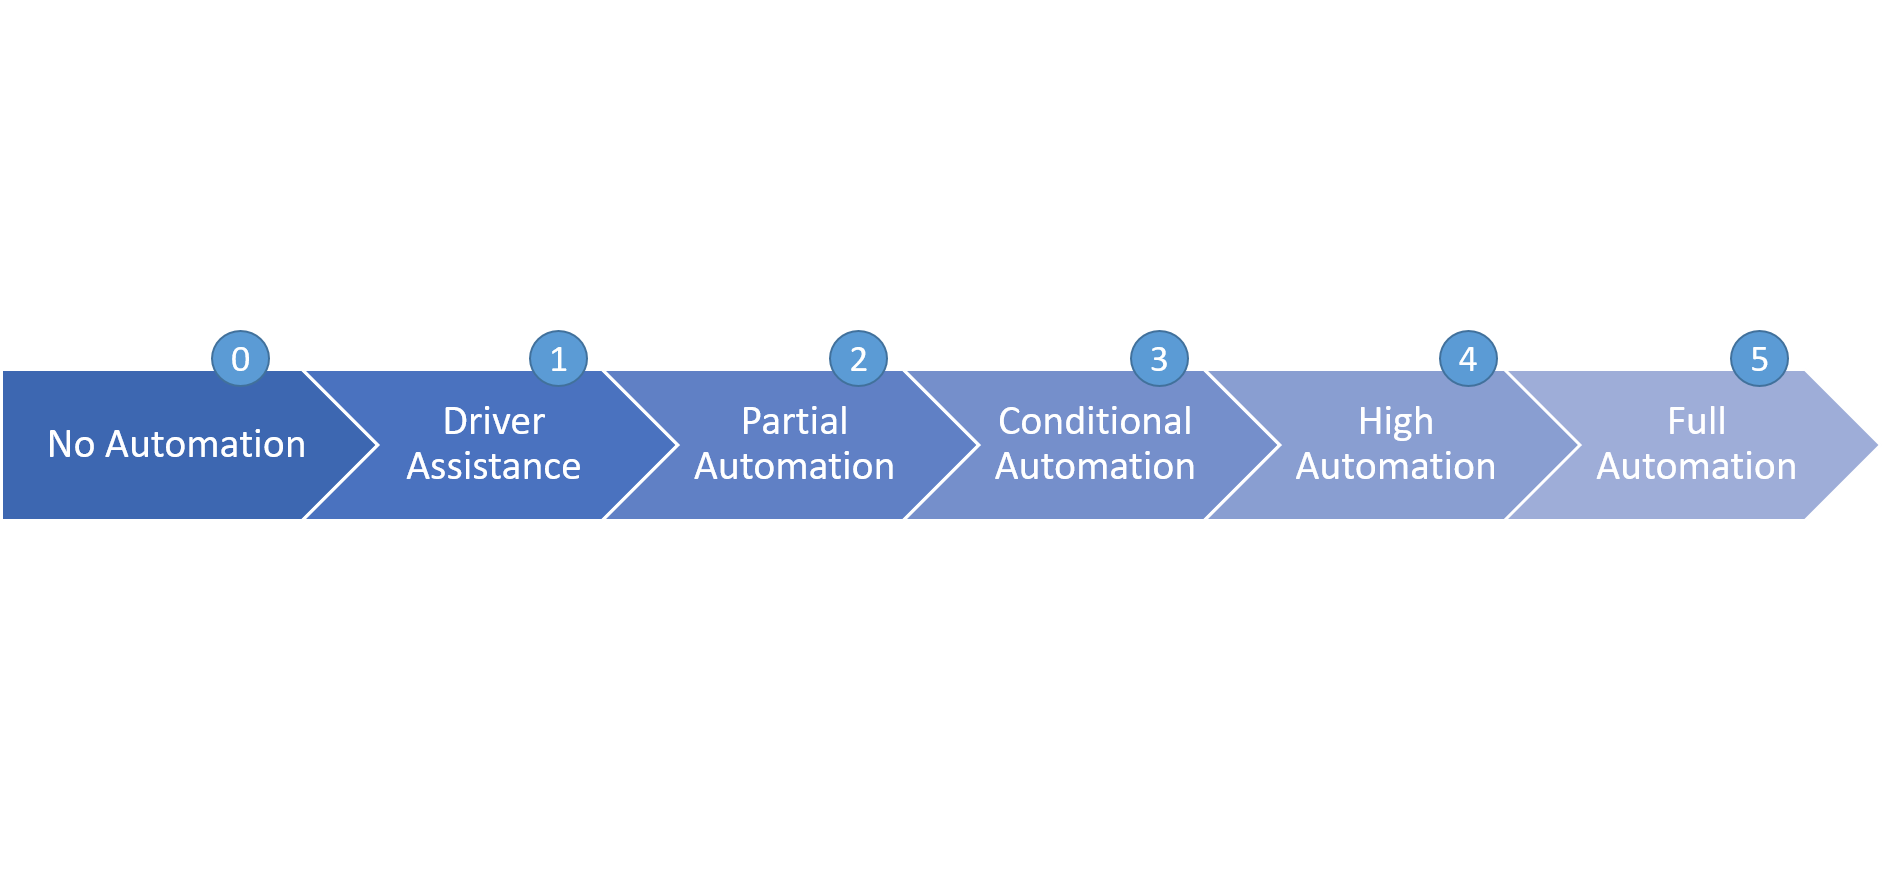
\includegraphics[scale=0.55]{imagens/diagrama_levels.png}
\caption{Levels of driving automation}
\label{fig:automation}
\end{figure}

\section{Problem Description}

This theme's problem is to create an architecture to detect objects along the roads combined with the distance measurement of these along the road. The first approach could be using a drone, but due to the battery conditions for long tests, it is not a good choice. Figure \ref{fig:tests} shown this problem. The goal is to track the position of the cars, even vehicles under the test (VUT) and traffic simulation data (TSV) along the road, and send this information to the command central (CC). 

\begin{figure}[H]
\centering
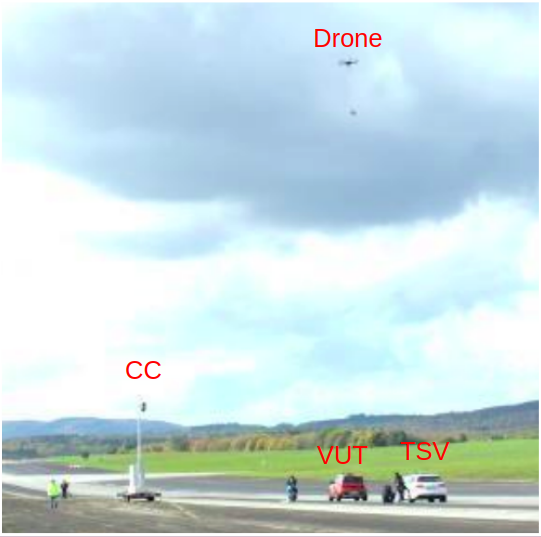
\includegraphics[scale=0.6]{imagens/proposal.png}
\caption{Modelling of the project using drones, where CC means command central, VUT is vehicle under the tests and TSV is traffic simulation vehicle.}
\label{fig:tests}
\end{figure}

\section{Objectives}

Create a framework able to detect objects as cars, trucks, motorcycles, pedestrians, and other strange obstacles along the road. With these capacities estimate the distance of this object along the way, this framework is necessary to work with a camera array.

\section{Published Works}

Along with developing this work, the author worked in several areas of computer sciences, particularly the data science domain, and always tried to keep the multidisciplinarity. These are my published works along my master degree:

\begin{enumerate}

\item \textbf{PRACIANO, BRUNO J. G.}; DE CALDAS FILHO, FRANCISCO L. ; E MARTINS, LUCAS M. C. ; DA CUNHA, DAYANNE F. ; DA SILVA, DANIEL ALVES ; DE SOUSA JÚNIOR, RAFAEL TIMÓTEO. SEGURANÇA DO AMBIENTE USANDO DISPOSITIVO IOT COM PROCESSAMENTO DISTRIBUÍDO. In: Atas da conferência IberoAmericana WWW/Internet 2019, 2019. Atas da conferência Ibero-Americana WWW/Internet 2019, 2019. p. 163

\item MARQUES, Angelica Alves da Cunha; \textbf{PRACIANO, Bruno Justino Garcia}. Researchers of the Brazilian archivistics scientific community in French international areas of interlocution Encontros Bibli: revista eletrônica de biblioteconomia e ciência da informação, Florianópolis, v. 25, p. 01-14, mar. 2020. ISSN 1518-2924. doi:https://doi.org/10.5007/1518-2924.2020.e65864.

\item CASTELINO, R. M.; MOREIRA, G. P.; \textbf{PRACIANO, BRUNO JUSTINO GARCIA}; SANTOS, GIOVANNI A.; WEICHENBERGER, L.; DE SOUSA, JR, RAFAEL T. Improving the accuracy of pedestrian detection in partially occluded or obstructed scenarios. In: 2020 10th International Conference on Advanced Computer Information Technologies, 2020, Deggendorf. 2020 10th International Conference on Advanced Computer Information Technologies, 2020. (to be published)

\item CANEDO, EDNA; PINHEIRO, GABRIEL; SOUSA JR., RAFAEL; RIBEIRO, RENATO; \textbf{PRACIANO, BRUNO}; LOPES DE MENDONÇA, FÁBIO. Front End Application Security: Proposal for a New Approach. In: 22nd International Conference on Enterprise Information Systems, 2020, Prague. Proceedings of the 22nd International Conference on Enterprise Information Systems, 2020. p. 233.

\item SOUSA JR., RAFAEL; LOPES DE MENDONÇA, FÁBIO; NZE, GEORGES; PINHEIRO, GABRIEL; \textbf{PRACIANO, BRUNO }; CANEDO, EDNA. Performance Evaluation of Software Defined Network Controllers. In: 10th International Conference on Cloud Computing and Services Science, 2020, Prague. Proceedings of the 10th International Conference on Cloud Computing and Services Science, 2020. p. 363.


\item SILVA, DANIEL ALVES DA; TORRES, JOSÉ ALBERTO SOUSA; PINHEIRO, ALEXANDRE; DE CALDAS FILHO, FRANCISCO L.; MENDONÇA, FABIO L. L.; \textbf{PRACIANO, BRUNO J. G}; KFOURI, GUILHERME OLIVEIRA; DE SOUSA, JR, RAFAEL T. Inference of driver behavior using correlated IoT data from the vehicle telemetry and the driver mobile phone. In: 2019 Federated Conference on Computer Science and Information Systems, 2019. org.crossref.xschema.\_1.Title@7d70270b, 2019. p. 487.

\item KFOURI, GUILHERME DE O. ; GONÇALVES, DANIEL G. V. ; DUTRA, BRUNO V. ; ALENCASTRO, JOÃO F. DE ; FILHO, FRANCISCO L. DE CALDAS ; MARTINS, LUCAS M. C. E ; \textbf{PRACIANO, BRUNO J. G.} ; ALBUQUERQUE, ROBSON DE O. ; JR, RAFAEL T. DE SOUSA . Design of a Distributed HIDS for IoT Backbone Components. In: 2019 Federated Conference on Computer Science and Information Systems, 2019. org.crossref.xschema.\_1.Title@7bad8b1f, 2019. p. 81.

\item DE MENDONCA, FABIO L. L.; DA CUNHA, DAYANNE F.; \textbf{PRACIANO, BRUNO J. G.}; DA ROSA ZANATTA, MATEUS; DA COSTA, JOAO PAULO C. L.; DE SOUSA, RAFAEL T. P2PIoT: A Peer-To-Peer Communication Model for the Internet of Things. In: 2019 Workshop on Communication Networks and Power Systems (WCNPS), 2019, Brasilia. 2019 Workshop on Communication Networks and Power Systems (WCNPS), 2019. p. 1.

\item BRANDAO, IURE V.; DA COSTA, JOAO PAULO C. L.; SANTOS, GIOVANNI A.; \textbf{PRACIANO, BRUNO J}. G.; JUNIOR, FRANCISCO C. M. D.; DE S. JUNIOR, RAFAEL T. Classification and predictive analysis of educational data to improve the quality of distance learning courses. In: 2019 Workshop on Communication Networks and Power Systems (WCNPS), 2019, Brasilia. 2019 Workshop on Communication Networks and Power Systems (WCNPS), 2019. p. 1.


\item DO NASCIMENTO SILVA, GERSON ; DE CALDAS FILHO, FRANCISCO LOPES ; DOS REIS, VINICIUS ELOY ; \textbf{PRACIANO, BRUNO JUSTINO }; LUSTOSA, JOÃO PAULO ; DE SOUSA JÚNIOR, RAFAEL TIMÓTEO . MODELO DE REDES NEURAIS ARTIFICIAIS EM SUPORTE TECNOLÓGICO À DETECÇÃO DE CARTEIS EM LICITAÇÕES PÚBLICAS. In: Atas da conferência IberoAmericana WWW/Internet 2019, 2019. Atas da conferência Ibero-Americana WWW/Internet 2019. p. 191.

\end{enumerate}

\section{Chapters Description}

This work is divided as follows: in Chapter 2, state of the art is presented, to support this work, once it is necessary to get a good part of the previous contributions in this research area. Chapter 3 presents the theoretical concepts to promote the understanding of this work. Since self-drive cars are a new trend topic is necessary to describe step by step about this essential to provide an excellent theoretical background. In Chapter 4, the proposed framework is shown, and mathematical modeling is presented. In Chapter 5, the results are discussed around the algorithm performance and the error for object detection position estimation. Finally, in Chapter 6, the conclusions are discussed regarding the experiments, and some future works are shown.


